\chapter{Development}
Initially, the algorithm should be able to take an existing non-empty graph as input. This graph can initially be seen as static and therefore HyperBall can perform a complete calculation on it. After HyperBall has completed, the calculated counters can be used as initial counters for the dynamic algorithm. For every insertion and deletion in the dynamic graph, these initial counters are manipulated. If an edge is added, nodes might reach more nodes than before and their counters should be raised. Similarly for deletions, if an edge is deleted, nodes might reach fewer nodes and their counters should be decreased.


\section{Dynamic graphs}

The ability to insert new nodes and edges (called entries in this section) to an existing graph is needed to achieve a dynamic graph. The graph files used by HyperBall are tightly compressed in a byte stream, which makes it an expensive operation to modify the graph at an arbitrary point. This makes it infeasible to insert every additional entry directly into the graph file. Instead, new entries can be stored in some other data structure.

The additional entries could either be stored in a high-level data structure or a byte stream. Keeping them in a high-level data structure will consume a significant amount of storage already at a low number of extra entries. A high-level data structure takes up more memory as each number is always the same size no matter what the value is. For example, the value 3 can be expressed by two bits but a high level integer always take a fixed amount of bits to express this.  Additionally, if each node has a structure containing the neighbors, a significant amount of space will be taken by the pointers to those structures. The compression of the graph is also lost when using a high-level structure.

If a byte stream is used, it is the same problem as the original. Even though this byte stream will be smaller, there will be a point where it is unreasonable to resize the stream and reposition the existing entries at each new entry. Regardless of which method is used, the extra entries and the original graph have to be merged into a new graph at some point. 

\subsection{Benchmark}
A benchmark was performed to compare the performance of a high level data structure and a byte stream, see figure \ref{fig:benchmarkByteStreamVsHighLevelTime}, \ref{fig:benchmarkByteStremVsHighLevelMemory}. The graph in-2004 was used, see appendix \ref{appendix4}. Figure \ref{fig:benchmarkByteStreamVsHighLevelTime} shows the time difference of adding edges and then performing a complete edge scan on the graph. It is evident in the figure that it is more efficient to use a high level data structure whenever edge additions are more common than edge scans and a byte stream when edge scans are more common. 

In figure \ref{fig:benchmarkByteStremVsHighLevelMemory} the memory difference can be seen. The high level data structure and the byte stream have the same space complexity, but the difference can be explained by the memory overhead used by the high level data structure. 

\begin{figure}[h]
\centering
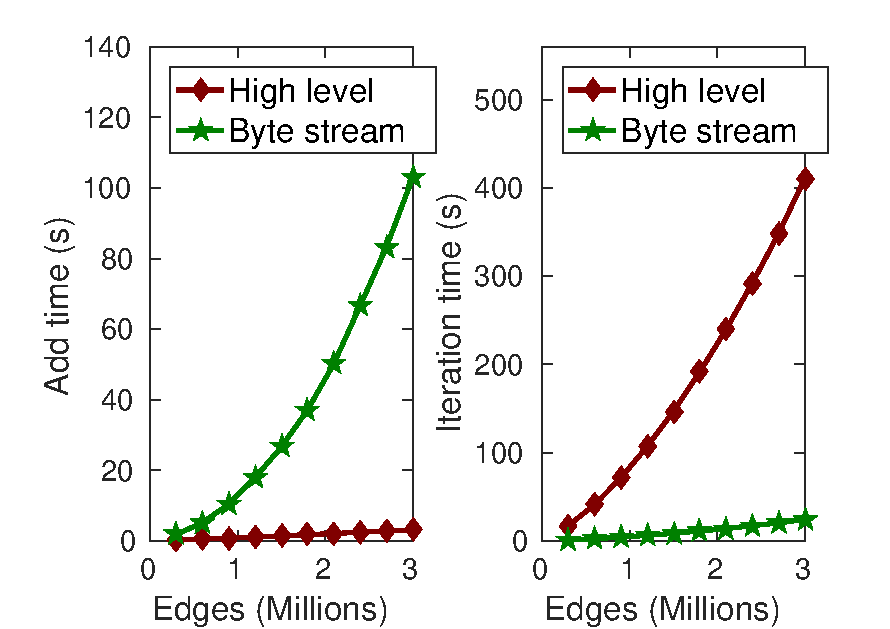
\includegraphics[]{benchmarkByteStreamVsHighLevelTime}    
\captionsetup{justification=centering}
\caption {Benchmark of time difference between high level structure and byte stream. }
\label{fig:benchmarkByteStreamVsHighLevelTime}
\end{figure}

\begin{figure}[h]
\centering
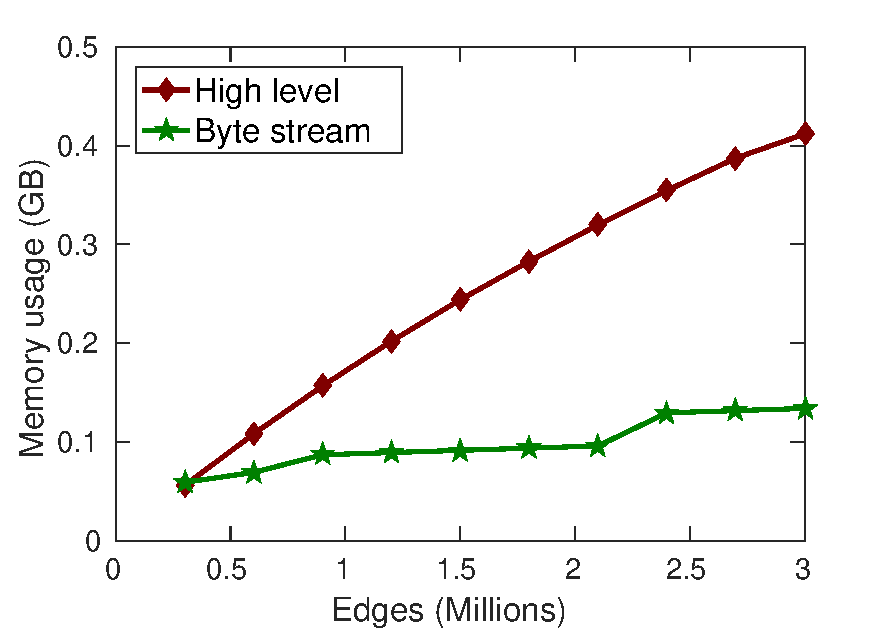
\includegraphics[]{benchmarkByteStremVsHighLevelMemory}    
\captionsetup{justification=centering}
\caption {Benchmark of memory usage between high level structure and byte stream. }
\label{fig:benchmarkByteStremVsHighLevelMemory}
\end{figure}


\subsection{Merging two graphs with webgraph}
The webgraph framework has a method for creating a new graph $G$ by taking the union of two sub graphs $G_1$ and $G_2$. The graph $G$ works by simultaneously reading from both the streams of $G_1$ and $G_2$ to produce the nodes and their neighbors. The sub graphs can be unions as well which means that an arbitrary number of graphs can be joined using this method. However, having lots of recursive unions create a large overhead in time when fetching nodes and edges. \cite{webgraph} 

The framework also supports writing a union-graph to disk as a new graph. Loading this new written graph removes the overhead of several recursive unions. As the graph express some arcs by references to previous arcs, the creation is slow and does not leverage any of the calculations already made by the existing graphs. Ignoring the references will make the graphs bigger but it increases the running time of the merge.

\subsection{Memory dependent merging}
To leverage the benefits of both high level structures and byte streams a mixture of both is used to achieve dynamic graphs. The original graph is kept as a byte buffer and the additional entries are saved in a high level structure. The high level structure was chosen as it has the fastest insertions. Each new bulk of edges is inserted into the high level structure. The union method of webgraph can then be used to union the high level structure and the original graph, creating a dynamic graph.

The overhead of recursive unions can be avoided by limiting the number of unions to one. By inserting each bulk insertion into the same high level structure, and keeping the original graph separated, the current union can be replaced by a new. However, the problem of the high memory overhead of using a high level structure still remains. 

The idea is to merge the graphs when the additional entries' memory usage, compared to the byte stream graph, reaches a certain ratio. The merged graph is stored and loaded as a byte stream. At this point, the additional edges are removed, as they are now part of the original graph. This resets the memory overhead of the high level data structure.


\subsubsection{Benchmark}
To find a suitable byte stream graph to additional memory usage ratio $r$, a benchmark was performed, comparing the time and space usage, see figure \ref{fig:benchmarkUnionVsStored}. The benchmark was performed on the In-2004 graph, see Appendix \ref{appendix4}. 1,000,000 edges were randomly generated and inserted into the graph in bulks of 5,000. The elapsed time measured is the time to insert the edges into the dynamic graph and then performing a complete edge scan. The memory measured is the graphs heap size. The plotted time values are the average of ten bulk insertions.

For reference, the benchmark compares a certain ratio with the extremes. With $r = \infty$ the additional entries are never merged with the original graph. This represents the optimal elapsed time. With $r = 0$, the graphs are always merged after each bulk insertion. This represents the optimal memory usage. By choosing $r = 8$, the benchmark shows that near optimality in both time and memory usage can be achieved. 

\begin{figure}[h]
\centering
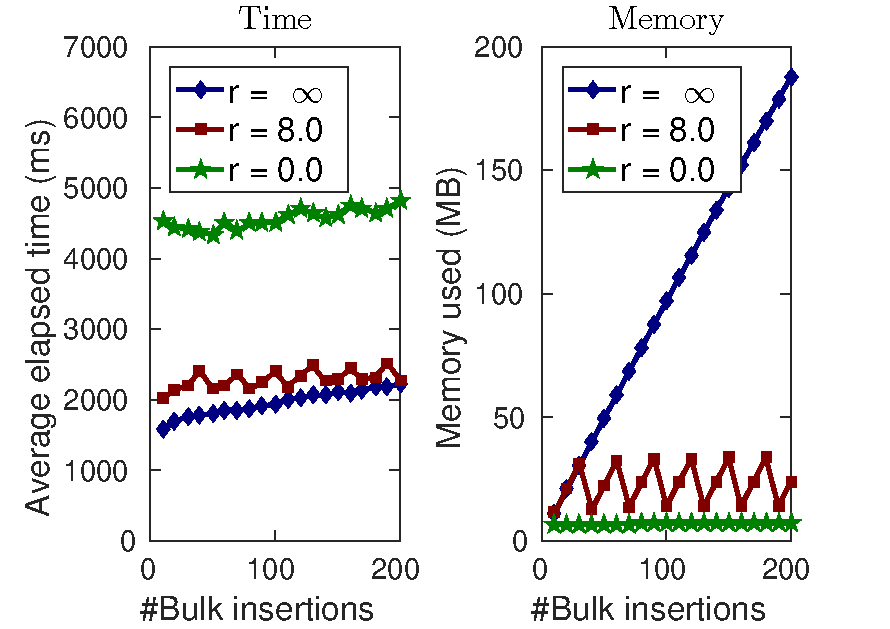
\includegraphics[]{benchmarkUnionVsStored}    
\captionsetup{justification=centering}
\caption {Benchmark of different union to stored memory ratio limits }
\label{fig:benchmarkUnionVsStored}
\end{figure}


\section{HyperLogLog resize}
After new nodes have been added to the graph, new counters have to be created for them. The initial counters retrieved by HyperBall are represented as an array of longs. This representation is kept as it has a very amount of wasted space usage. It also minimized the number of objects created on the heap. But as new counters are needed, the array must be resized. For this, a geometric expansion is used as it gives $O(1)$ amortized time per insertion \cite{dynamicarrays}. Amortized time is the required time averaged over the elements operated on. In the geometric expansion the array capacity is increased by a factor. This is how the standard implementation of ArrayList in Java is dynamically increased. A larger factor implies an on average small number of copies per inserted elements but a high amount of unused space. The amortized number of copies per inserted element for a factor $r$ is roughly $\frac{1}{(r-1)}$ and the average unused space is $\log(r)*\frac{r}{(r-1)} - 1$. \cite{dynamicarrays}

Under the assumption that the graph expands slowly relative to its size, resizing events will be sparse and a large factor would mainly imply a large amount of unused memory. Therefore, it is more beneficial to let the array increase by a small factor. With the factor $r = 1.1$, an average of $4.8$\% space is unused and every element will on average be copied $10$ times.

\section{Updating counters}

After an edge has been added to the graph, the next step is to update the counters of all nodes affected by the insertion. Figure \ref{fig:collect_and_propagate} will be used as an example. The black arrows are edges. The green circles are the counters produced by the collection steps. The red and orange arrows are the propagation step. Let $e = (2,4)$ be an edge added to the graph. All the nodes reachable from $4$ have to be propagated to the nodes that can now reach $4$ via $2$. Propagation means that all newly reachable nodes are hashed and inserted into the counters of the nodes that now reach them. This is performed in two phases, the collecting-BFS and the propagating-BFS.

The collecting-BFS is responsible for retrieving which nodes $2$ can reach. The collecting-BFS performs a BFS in the graph from $4$. For every level $i$ in the BFS, all nodes in the current frontier in the BFS are added into a HyperLogLog counter, visualized as the green circles in figure \ref{fig:collect_and_propagate}. This counter represents all nodes that $4$ reached in $i$ steps. The collecting-BFS completes at level $h-1$ and returns a $h$ long list of counters. The $h$'th step is not needed as not even $2$ can reach level $h$.

The propagation-BFS is responsible for updating the counters of all nodes that now reach $4$, as they might have changed by the insertion. To find all nodes that can reach $4$, a BFS is performed from $2$ in the transpose of the graph. For every level $i$ in the BFS, the frontier of nodes in the BFS can reach all nodes that the collecting-BFS reached in $h-1-i$ steps. To update the counters of the nodes at level $i$, the current counters of the nodes are merged with the counters from collection steps $\leq h-1-i$ retrieved in the collecting-BFS. The propagation-BFS stops after $h-1$ steps after which all affected node counters have been updated.\\

\begin{figure}[h]
\centering
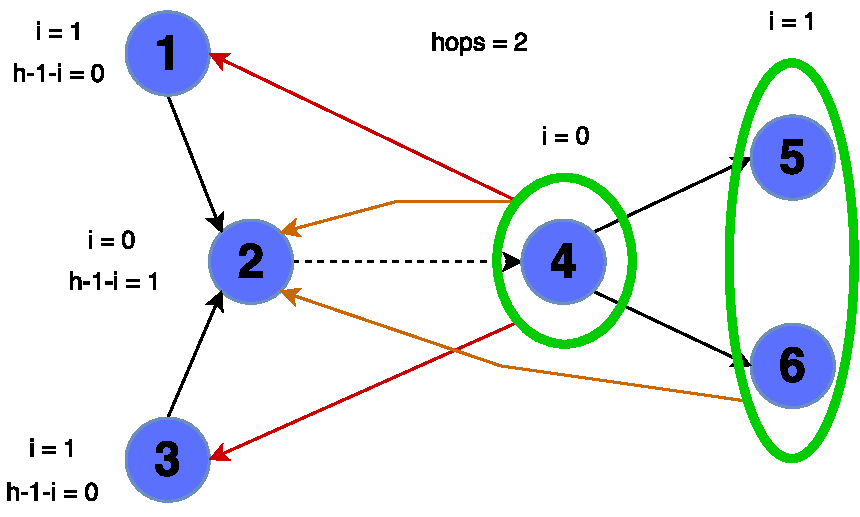
\includegraphics[]{trivial_collect_and_propagate}    
\captionsetup{justification=centering}
\caption {Visualization of the collect and propagate steps}
\label{fig:collect_and_propagate}
\end{figure}

\begin{theorem} The two-BFS algorithm yields node counters identical to a HyperANF recalculation.

\begin{proof}Let $S(v)_i$ be the set of nodes added to the counter of $v$ after $i$ edges have been inserted.\\

\noindent\textit{Base case:} $i = 0)$ As the algorithm uses HyperANF to calculate the initial counters, $S_{2bfs}(v)_0 = S_{hanf}(v)_0$.\\

\noindent\textit{Inductive hypothesis: } $\forall i \leq n : S_{2bfs}(v)_i = S_{hanf}(v)_i$.\\

\noindent\textit{Inductive case: } $n + 1)$ Let $N(v)_i = S(v)_i \backslash S(v)_{i-1}$.  $S_{hanf}(v)_{n+1} = \{ u : dist(u,v) \leq h \}$ and $S_{2bfs}(v)_{n+1} = S_{2bfs}(v)_{n} \cup N_{2bfs}(v)_{n+1}$. By the two-BFS algorithm, all nodes within h distance from an edge insertion are collected and propagated, hence $N_{2bfs}(v)_{n+1} = N_{hanf}(v)_{n+1}$. By the inductive hypothesis: $S_{2bfs}(v)_{n+1} = S_{2bfs}(v)_n \cup N_{2bfs}(v)_{n+1} = S_{hanf}(v)_n \cup N_{hanf}(v)_{n+1} = S_{hanf}(v)_{n+1}$.
\end{proof}
\end{theorem}

\subsection{Optimized Breadth-first search}

A problem with the two phase algorithm described above is that it only supports single insertions at a time. Instead of adding each edge separately, they can be bulked into a set of edges to add. By bulking the edges several BFS's can be performed at the same time. 

The algorithm MS-BFS \cite{msbfs} does several BFS's at the same time very effectively and will be used in the algorithm. The standard BFS and MS-BFS was compared by performing a benchmark, see figure \ref{fig:benchmarkbfs}. Both algorithms had to perform breadth first searches from a certain number of source nodes and for a specified number of steps. The graph It-2004, see Appendix \ref{appendix4}, was used. In figure \ref{fig:benchmarkbfs} the ratio between the total time for the standard bfs and the MS-BFS is plotted. Note that the y axis scale is logarithmic. The dashed line indicates where both algorithms are equally fast. MS-BFS is faster for all points above the dashed line and the standard BFS is faster for all points below it. From the figure it is clear that the standard BFS is faster for a small amount of steps but the speed ratio is exponentially increased in favor of MS-BFS as the steps increase. After $3$ steps, MS-BFS outperforms the standard BFS, even for a relatively small amount of sources. The standard BFS was up to $60$ times slower in our benchmark.

\begin{figure}[h]
\centering
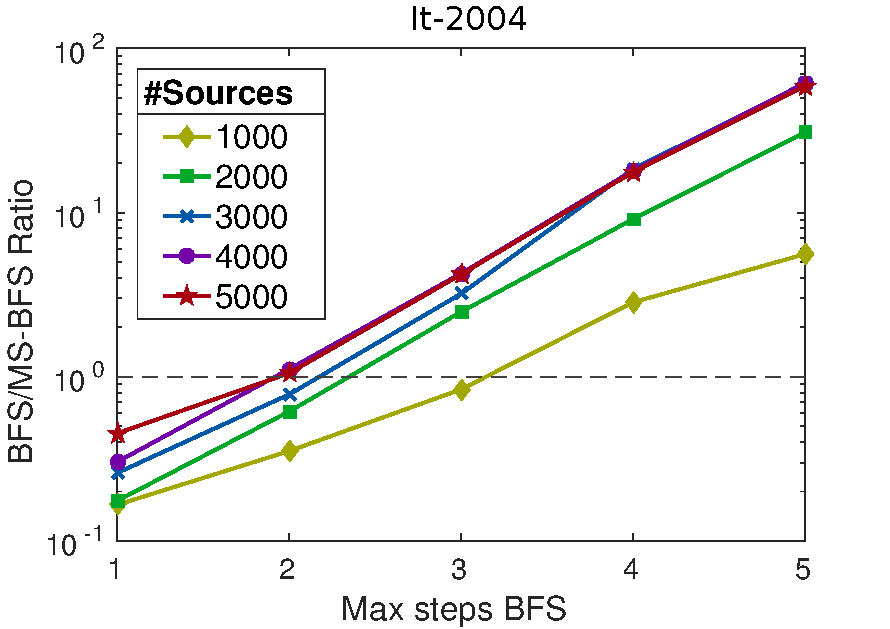
\includegraphics{benchmarkBfs}    
\captionsetup{justification=centering}
\caption {Comparison standard BFS and MSBFS}
\label{fig:benchmarkbfs}
\end{figure}

\subsubsection{Visitors}
In order to prune paths in the BFS, there needs to be a way to stop the individual BFS's. This was solved by implementing a method to pass the MS-BFS a visitor function (not related to the common Visitor design pattern). The visitor will be called every time a group of BFS's have reached a node. The group of BFS's that reached the node is represented as a list of bits and is passed to the visitor. If the visitor wants to stop the propagation of a BFS from this node it can clear the corresponding bit. No modifications to the algorithm needs to be done as MS-BFS already use a list of bits to propagate the BFS's.

\subsubsection{Travelers}
It can be desirable to send data along the BFS's. For this, a new concept called Travelers was implemented. The purpose of the traveler is to bring initial data from the BFS's and merge the data if several BFS's reach a node at the same time. This may prevent calculations that would otherwise need to be done in all or many of the visitors by removing the need to loop through which source nodes that reached the node. Travelers have to be able to merge to not increase the space complexity of the algorithm. The travelers are then passed to the visitors so they can use the data provided by the travelers. 

\subsubsection{Extended algorithm}

The extended algorithm is presented in figure \ref{fig:extended_ms-bfs_algorithm}. It has only slight modifications compared to the algorithm in section 4.1.1 from \cite{msbfs}. The visitor is called on line 12. The neighbors are not inspected if the visitor returns an empty set. The travelers are merged at lines 16 to 19. If the neighbor will be visited from other nodes, i.e. the $visitNext$ bits are not empty, the existing traveler are merged with the traveler from the current node.

\begin{figure}[h]
    \begin{lstlisting}[mathescape]
Input: $G$, $B$, $S$, $V$, $T$
for each $b_i \in B$
    $seen[ s_i ] \leftarrow 1 << b_i$
    $visit[ s_i ] \leftarrow 1 << b_i$
for each $t_i \in T$
    $travelers[s_i] \leftarrow t_i $
reset $visitNext$

while $visit \neq \emptyset$
    for $i = 1, ... , N$
        if $visit[v_i] = \emptyset$, skip
        $visit[v_i] \leftarrow V(v_i,visit[v_i],travelers[v_i])$
        if $visit[v_i] = \emptyset$, skip
        for each $n \in neighbors[v_i]$
            $traveler \leftarrow travelers[v_i]$
            if $visitNext[n] \neq \emptyset$
                $traveler \leftarrow traveler.merge(travelersNext[n])$
            $travelersNext[n] \leftarrow traveler$
            $visitNext[n] \leftarrow visitNext[n] | visit[v_i]$
            
        for $i = 1, ... , N$
            if $visitNext[v_i] = \emptyset$, skip
            $visitNext[v_i] \leftarrow visitNext[v_i] \& \sim seen[v_i]$
            $seen[v_i] \leftarrow seen[v_i] | visitNext[v_i]$
    $visit \leftarrow visitNext$
    reset $visitNext$
    $travelers \leftarrow travelersNext$
    reset $travelersNext$
    \end{lstlisting}
    \caption{Extended MS-BFS algorithm}
    \label{fig:extended_ms-bfs_algorithm}
\end{figure}


\section{Node history}

MS-BFS speeds up the algorithm significantly, but further optimizations can be done to the individual BFS's. To update a counter, the algorithm has to do two BFS's for every edge added. A large portion of the time spent by the algorithm will be doing these BFS's. Therefore, the ability to prune BFS's early would imply a large time improvement of the run time. Currently, the collecting-BFS must traverse the graph $h$ steps to gather all data needed. This is because every node only keeps track of its registers resulted by a search in $h$ steps. If all nodes also keeps track of its registers in $h-1$ steps, then the collecting-BFS would only need to traverse $h-1$ steps. This as in the $h-1$'th step the collecting-BFS can use the $h-1$ history of all nodes to calculate the $h$'th step. For every extra history level added, the collecting-BFS can stop one step earlier. So by saving every history level of all nodes, the collecting-BFS only needs to visit the immediate neighbors of a new node $v$ to be able to calculate the counter of $v$. 

During the HyperBall phase of the algorithm, the intermediate counters in HyperBall can be used to calculate all history levels of all nodes. HyperBall works in iterations, synchronizing all nodes between every iteration. During the $i$'th synchronization, the counters will represent the $i$'th level of all nodes history. So instead of only using the last level from HyperBall, all levels are saved. The $h'th$ level will be referred to as the top counter and level $0$ to $(h-1)$ as history counters. All levels combined will be referred as counter collection.  

Every node now has a list of its history which has to be updated with every edge update. For an edge $e = (u,v)$ inserted, the collecting-BFS has to gather the node history from all neighbors of $v$ and merge them into one. The merged history together with $v$ itself added to them becomes $v$'s own history and counter. Then the propagation-BFS has to propagate this history in the transpose of the graph. These merging operations can be performed during the current BFS's and does not affect the time complexity of the BFS's.

With node history the algorithm has $O(hn \log \log n)$ space complexity, as the top counter uses $O(n \log \log n)$ and the history counters use $O((h-1)n \log \log n)$. To insert an edge $e = (u,v)$, the two previous BFS's used $O(m)$ operations per BFS but with node history the collecting-BFS use $O(d^+(v))$ operations, where $d^+(v)$ is the out degree of node $v$. The time complexity of the node history version is then $O(m + d^+(v))$. In practice, this means a large improvement as it often holds that $d^+(v) << m$.

Node history speeds up the algorithm but also uses extra space that, for large graphs, can be quite extensive. To create an algorithm that balances the gained speed versus the extra memory usage, the history could be saved for only a subset of nodes. These nodes should be chosen so that as few nodes as possible need to save their history while keeping the BFS distance as short as possible. The algorithm to determine these nodes have to be very fast to avoid affecting the running time of the algorithm. It would also have to be dynamic to be able to continuously determine which nodes that should be included in the set.

\subsection{Vertex cover}
\label{sec:vertex_cover}
One way to determine which nodes that should keep their history is to use the nodes that are in a minimum vertex cover $VC$. Only saving the node history of nodes that are part of the $VC$ can significantly improve space usage, yet the BFS can still be bounded.

The top counter still needs to contain counters for all nodes so the space complexity of the top counter is still $O(n\log \log n)$. As the history counters only include counters of nodes in the $VC$, the history counters space complexity is reduced from $O((h-1)n \log \log n)$ to $O((h-1)|VC| \log \log n)$. In total, the node history use $O(((h-1)|VC| + n )\log \log n)$ space.

The trick here is that for all nodes $u$, it holds that $\forall u \in V: u \in VC \vee \forall e = (u,v) : v \in VC$. Then, when the collecting-BFS searches from a node $v$ it will take at most one step for nodes not in the vertex cover and two steps for nodes in the vertex cover until they reach a frontier of only nodes in the vertex cover. From this frontier, the collecting-BFS can calculate $v$'s history and counter by merging the frontiers collecting histories. The collection-BFS is now bounded by two steps, resulting in $O(d^+(v) + \sum_{u \in s(v)}{d^+(u)})$ operations. $s(v)$ is the successors of $v$.

\subsubsection{Dynamic minimum vertex cover}
There is a requirement to, at all times, keep track of which nodes are in the vertex cover. This requires a fully dynamic minimum vertex cover algorithm. However, as minimum vertex cover is NP-complete, approximation algorithms must be used. The choice of fully dynamic approximate minimum vertex cover algorithm depends on the ratio between the number of insertions and deletions. A simple greedy algorithm can maintain a $2$-approximation in $O(1)$ time per insertion and $O(n)$ time per deletion \cite{2appdynvc}, while an algorithm that partition the nodes can maintain the same approximation in $O(\log n )$ amortized time per insertion and deletion \cite{2appdynvclogn}. In our case, deletions will be very sparse in the data stream, which is why the greedy algorithm was chosen. The greedy algorithm also have the property that if a deleted edge was not part of the maximal matching previously, it deletes the edge in $O(1)$ operations. For dense graphs, only a small amount of the edges will be in the maximal matching, which makes the greedy algorithm perform quickly in deletions as well. 

 
\subsubsection{Directed graphs}
As the standard minimum vertex cover problem is defined for undirected graphs the problem have to be slightly modified. The new problem description is as follows; given a directed graph $G = (V,E)$, select a minimum cardinality subset $V' \subseteq V$ such that $\forall e = (u,v) \in E, u \in V' \vee v \in V'$. The problem is still NP-complete as undirected graphs are a special case of directed graphs. 

By the same reasoning as in the undirected case, a maximal matching is a $2$-approximation of the generalized problem. The greedy algorithm needs to be modified to support directed edges. The only case affected is when an edge in the maximal matching is deleted. Let $e = (u,v)$ be a deleted edge. Previously, the algorithm removed both $u,v$ from the vertex cover and then scanned the outgoing edges from $u,v$ for edges uncovered due to the removal. With directed edges, both incoming and outgoing edges must be verified. This is solved by scanning the outgoing edges of $u,v$ in both the original graph and the transpose of it. The original graph will give the outgoing edges of $u,v$ and the transpose the incoming.

\subsubsection{Benchmark insertions}
The selected greedy algorithm was benchmarked with the it-2004 graph, see Appendix \ref{appendix4}. Starting with an empty graph, every edge was sequentially inserted from it-2004 into the dynamic vertex cover. Both the time and heap size was measured over the number of inserted edges, see figure \ref{fig:benchmarkDvcInsertion}. This shows roughly 29.5 million inserted edges per second. The memory used mainly depends on the number of nodes. The heap size increased to 0.33GB. 0.33GB equals 354,334,801 bytes, making it an average of 8 bytes per node. 

\begin{figure}[h]
\centering
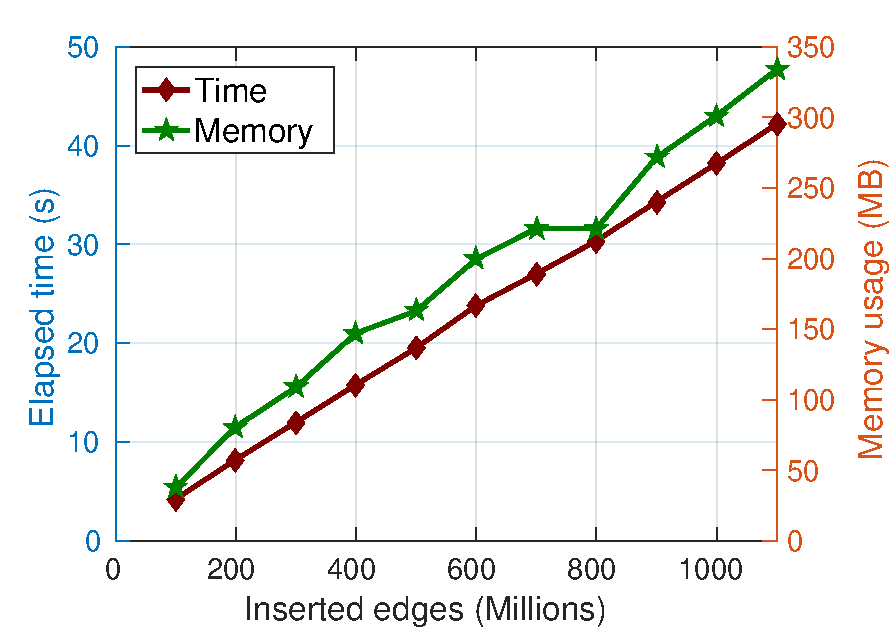
\includegraphics[]{benchmarkDvcInsertion}    
\captionsetup{justification=centering}
\caption {Benchmark of sequential insertions in 2-approximate dynamic vertex cover}
\label{fig:benchmarkDvcInsertion}
\end{figure}

\subsubsection{Benchmark deletions}
To test the performance of sequentially deleting edges the it-2004 graph was used, see Appendix \ref{appendix4}. The test was performed by first inserting all edges into the dynamic vertex cover and then sequentially delete them, see figure \ref{fig:benchmarkDvcDeletions}. All 1,150,725,436 edges were deleted in 220 seconds, giving a performance of 5,000,000 deleted edges per second. The heap usage is not plotted in the figure, as the algorithm is not designed to down size the allocated memory for the vertex cover after deletions. 

\begin{figure}[h]
\centering
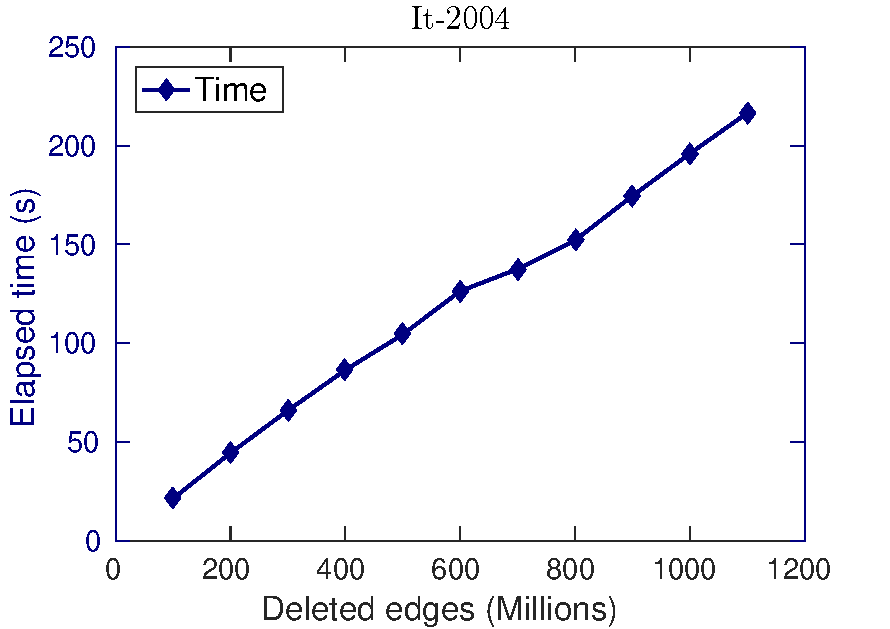
\includegraphics[]{benchmarkDvcDeletions}    
\captionsetup{justification=centering}
\caption {Benchmark of sequential deletions in 2-approximate dynamic vertex cover}
\label{fig:benchmarkDvcDeletions}
\end{figure}


\section{DANF}
\subsection{Edge insertion}

Edge insertion in DANF is divided into four steps. The first step is checking if a new edge contains any new nodes. New nodes are added to the graph and the top counter is, if necessary, resized to fit new counters of the new nodes. The second step is to check if any new node needs to be added into the vertex cover. For all new nodes in the vertex cover, memory is allocated in the history counters. The third step is calculating the history of the nodes added to the vertex cover. Lastly, the new history is propagated with a BFS in the transpose of the graph to update the counters of nodes affected by the insertion. After these four steps all nodes will have an approximate neighborhood function in their top counters and all nodes in the vertex cover will have their history counters updated. 

\subsubsection{Partial history calculation}
When a bulk of edges are inserted, the vertex cover needs to be modified and the histories updated. Using a maximal matching \cite{2appdynvc}, which does not delete any nodes upon insertion, the collecting-BFS can be upper bound to search at most one level to generate the partial history. For every node added to the vertex cover, the collecting-BFS only needs to retrieve the history that the node would have had before the current bulk insertion. The remaining of the node history will be propagated by the propagating-BFS.

The collecting-BFS of node $v$ looks through all its neighbors that are in the vertex cover and adds their history to its own. For this, only $O(d^+(v))$ operations are needed, which is an improvement to the time complexity stated in \ref{sec:vertex_cover}. \\

\begin{lemma} Only one BFS level is needed to collect the history a node $v$ would have after insertion $p$ during insertion $p+1$. 
\label{lemma:partial_history_calculation}

\begin{proof} Given a node $v$ whose history should be calculated for insertion $p+1$:\\

\noindent\textit{Fact:} It holds that $v \in VC \vee \forall e = (v,u) : u \in VC$.

\noindent\textit{Assumption:} The history of the nodes in the vertex cover is correct after insertion $p$.\\ 

\noindent Let $N_p(v,h) = \{v\}\bigcup\limits_{u \in s_p(v)} N_p(u,h-1) $ be the correct counter of $v$ between insertion $p$ and $p+1$, where $s_p(v)$ is the successors of $v$ in step $p$. Let $H_p(v,h) = \{v\}\cup\bigcup\limits_{u\in s_{p}(v)}N_{p-1}(u,h-1)$ be the calculated counter. Let $n_p(v)=s_p(v)\backslash s_{p-1}(v)$\\


\noindent As no edges are removed: 
$s_p(v) \subseteq s_{p+1}(v)$.\\ 
$H_{p+1}(v,h) = \{v\}\bigcup\limits_{u\in s_{p+1}(v)}N_{p}(u,h-1) = \{v\}\bigcup\limits_{u\in s_{p}(v)}(N_{p}(u,h-1)) \bigcup\limits_{u\in n_{p+1}(v)}(N_{p}(u,h-1)) \supseteq $\\ $\{v\}\bigcup\limits_{u \in s_p(v)} N(u,h-1) = N_p(v,h)$. \\

\noindent As $N_p(v,h)$ is a subset of $H_{p+1}(v,h)$, $H_{p+1}(v,h)$ must contain all elements in $N_p(v,h)$. As $H_{p+1}(v,h)$ only uses the history of its neighbors, it only needs one BFS level.

\end{proof} 
\end{lemma}

\subsubsection{History propagation}

When a new edge $e = (u,v)$ is added to the graph, many nodes that has a path to $u$ will contain outdated history. The algorithm works by propagating the history of $v$ through the transpose of the graph. If $v$ is not in the vertex cover, the history needs to be calculated from the neighbor nodes. The algorithm is presented in pseudo code, see figure \ref{fig:history_propagation_algorithm}.

\begin{figure}[h]
    \begin{lstlisting}[mathescape]
e = (u,v) //Edge to add
if(isInVertexCover(v))
    H$_v$ = H(v);
else
    H$_v$ = union of the history of the neighbor nodes;
In BFS; source: u, current node: z, at depth: d{
    d = d+1;  // The BFS is performed from u so the actual depth 
              // (from v) is one higher
    if(isInVertexCover(z)){
        foreach 0 $\leq$ i $<$ h+1-d{
            H(z,i+d).union(H$_v$(i));
        }
    }else{
        H(z,h).union(H$_v$(h-d));
    }
}
    \end{lstlisting}
    \caption{History propagation}
    \label{fig:history_propagation_algorithm}
\end{figure}

To speed up the algorithm, it needs to be modified to handle several edges at once. In this case the traveler support of the MS-BFS algorithm can be used. This means that the data provided by the traveler can be used instead of looping through all the source nodes. The travelers will contain the counter registers of their respective source node. When the travelers merge they can take the union of their registers. They also only need to keep the $h+1-depth$ top-most counters as the others won't reach further anyway. In the visitor the data from the traveler is joined with the existing counters of the visited nodes. The merge function for the traveler is constructed as in figure \ref{fig:history_propagation_traveler}.

\begin{figure}[h]
    \begin{lstlisting}[mathescape]
Input: t1,t2 = travelers to merge (HyperLogLog counters)
       d = depth of the BFS
Output: a new traveler
tOut = t1.clone
foreach 0 $\leq$ i $<$ h+1-d{
    tOut$_i$ = tOut$_i \cup $t2$_i$
}
return tOut
    \end{lstlisting}
    \caption{History propagation traveler}
    \label{fig:history_propagation_traveler}
\end{figure}

The visitors only have to be slightly modified to make use of this traveler. The only difference is that the visitor use the counter history from the traveler data instead of taking it from the source nodes.

Given that the partial history calculation makes sure that all nodes in the vertex cover has the history it would have before the current insertion, it can be proven that all nodes will have the correct history after the propagation step. \\

\begin{lemma} After an insertion $p+1$ all nodes have had all reachable nodes added to their counters.
\label{lemma:propagation}

\begin{proof}

\noindent\textit{Assumption 1: } The history of the nodes in the vertex cover has the history they would have after insertion $p$. \\

\noindent Take any two nodes $u,v$ where $u$ reach $v$ in at most $h$ steps. In insertion $p+1$ there are two cases. \\

\noindent\textbf{$u$ reached $v$ in insertion $p$}) By assumption 1 it holds that the history of $u$ is the same as it would be after insertion $p$, hence $v$ has been added to the counter of $u$.\\

\noindent\textbf{$u$ did not reach $v$ in update $p$}) As $u$ reach $v$ in update $p+1$, there must be a path $P$ from $u$ to $v$ where an edge has been added. Let $e = (a,b) \in P$ be the new edge of maximum hops from $u$. As $u$ reach $v$ in at most $h$ steps it holds that $|P| \leq h$.
As there are no more new edges between $b$ and $v$, combined with assumption 1 ($b$ has the history it would have after insertion $p$), $b$ will contain $v$. By the algorithm, the propagation step will traverse $h$ steps from $b$ and as 
$|P_{u \rightarrow b}| \leq |P| \leq h$ the propagation from $b$ will have reached $u$ and added $v$ to its counter. 

\end{proof}
\end{lemma}

\begin{theorem}
The history and counters of all nodes will be correct after every insertion.\\

\begin{proof} This will be proved by induction. Let $p$ be the number of edge insertions.\\

\noindent\textit{Base case:} $p = 0)$ The initial state is produced by HyperANF which has been proven to be correct.\\

\noindent\textit{Induction Hypothesis:} The history of all nodes are correct after $p$ insertions.\\

\iffalse
Given that the history of all nodes are correct after insertion $p$, they will be correct after insertion $p+1$.\\
\fi

\noindent\textit{Induction case:}
Running the partial history calculation is allowed, as the assumption is fulfilled by the induction hypothesis (\ref{lemma:partial_history_calculation}). The history propagation may then be run as the partial history calculation fulfills the assumption (\ref{lemma:propagation}). This means that the history of all nodes are now correct. 

\end{proof}
\end{theorem}


\subsubsection{Benchmark}
\todo{Write something about here}, see figure \ref{fig:benchmarkDanfVsTrivial}.


\begin{figure}[h]
\centering
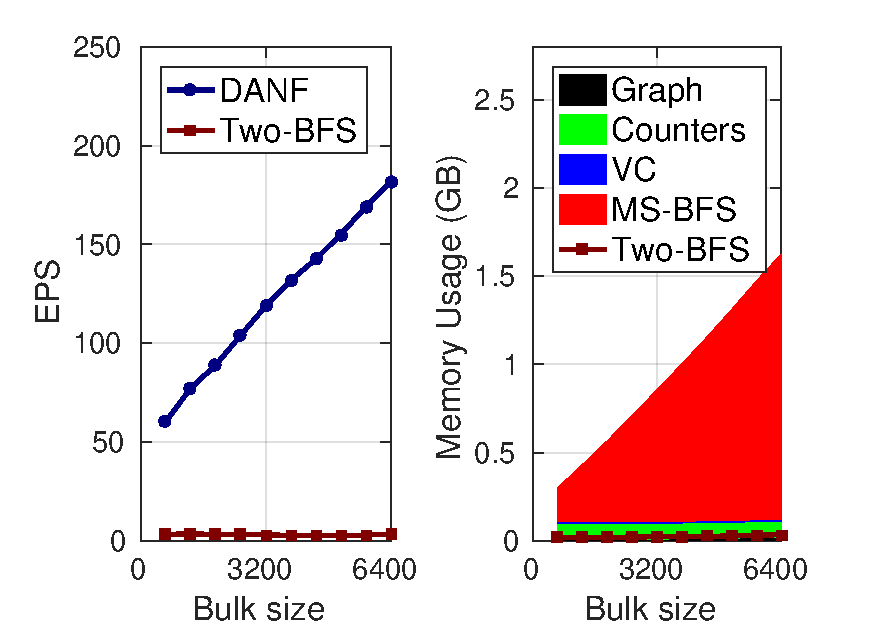
\includegraphics[]{benchmarkDanfVsTrivial}    
\captionsetup{justification=centering}
\caption {Benchmark of Danf compared to a trivial implementation}
\label{fig:benchmarkDanfVsTrivial}
\end{figure}
